\documentclass[12pt]{article}
%\renewcommand\normalsize{\fontsize{10pt}{12pt}\selectfont}
\usepackage{graphicx} % Required for inserting images
\usepackage[left=2cm,right=2cm,top=2cm,bottom=1.5cm]{geometry}
\usepackage{wrapfig}
%\pagestyle{empty} 

\title{Entropy}
%\author{Dennis Wilkinson}
%\date{March 31 2025; due Monday April 7}

\begin{document}

\setlength{\parindent}{0pt}
\setlength{\parskip}{3mm}

FS1 Wilkinson - Energy, irreversibility, and entropy

1. \underline{Energy}

To get to entropy, it's helpful to first review energy, and even before that, basic mechanics and Newton's 2nd law $F=ma$. Of course, $F=ma$ is at the heart of classical physics because it allows us, in theory, to understand any motion. Objects exert forces on each other depending on their relative positions; as a result of the forces, each object accelerates, changing its position, which changes the force it exerts on the other objects. That's it; classically, that's how everything happens. (Today, we understand that this picture - where force is the key concept - is only an approximation to how things work on a small scale; but we'll worry about that later.)

Okay, are we done? No, because (leaving aside the modern revelation that the classical Newtonian picture doesn't really work at small scales) unfortunately, $F=ma$ is difficult or impossible to apply in many cases. For example, consider a pole vaulter who wants to complete a vault. He needs to eat/breathe/drink, metabolize the food/air/water, get himself to the track, run down the runway at the right speed, plant the pole, jump off the ground, bend the pole back and have it snap him upward at the right angle, push off the pole, contort his body to just make it over the bar, then adjust again as he falls into the pit and is stopped. All of these steps involve $F=ma$; but, at such a complex level that it would be intractable and pointless to try to go through the calculations. Or, in a somewhat simpler case, we heat up some steam, and have it push a piston to operate a machine. No one would attempt to calculate the position and acceleration of all the steam molecules during this process! Even for a system of one sun and two planets interacting only by gravity, with no friction and air resistance to complicate matters - the famous three-body problem - it's impossible to use $F=ma$ to get a perfectly exact analytic solution in most cases.

The development of the concept of energy was a key step in understanding most real-world systems.  Though it took brilliant people a long time to understand and organize the formalism, in hindsight, it's pretty simple: for an object subject to force $\vec{F}(\vec{x})$, we just see what changes when the Newton $\vec{F}=m\vec{a}$ interaction persists as the object moves through distance $\vec{\Delta x}$. Mathematically, this is encoded by multiplying both sides of the equation by $\vec{\Delta x}$ (a dot product, actually):
\begin{equation}
    \vec{F}\cdot \vec{\Delta x} =  m\vec{a}\cdot\vec{\Delta x}.
\end{equation}
Whatever change the left side of this equation is describing, it's reflected by an equal change in the right side.  If the forces vary continuously, it's no problem; we just use calculus and consider infinitesimally small changes $d\vec{x}$, and the equality still holds.

How should we interpret this equality? Well, in class and your homework, you saw that the right side reduces to a change in $\frac{1}{2}mv^2$, which we call \textit{\textbf{kinetic energy}} or KE, the energy of motion. 

As for the left side, it can be viewed through two different lenses. From the perspective of the object, it describes how the forces affecting the object change as the object moves. From this perspective, we call it \textit{\textbf{potential energy}} or PE, because the object is moving to a new position where there may be more (or less) force on it, giving it more (or less) potential for future movement. And so we say that $\Delta$PE=$\Delta$KE.

A second interpretation of the left side of equation (1) is that some force $F$ is acting on our object, moving it through a distance $\Delta x$. When viewed from the outside in this way, this quantity is called \textbf{\textit{work}}, $W$, and we get that $W=\Delta$KE. This is known as the work-energy theorem. 

Here's a problem to illustrate work and energy.

\textbf{Problem 1.} An object of mass $m$ falls from a height $h$ under the influence of gravity; we ignore air resistance. 

\textbf{a.} Under the PE interpretation, we have PE being lost as the object falls. The KE when the box hits the ground equals the PE lost. Use PE=$mgh$ to show that the box's speed when it hits is $v=\sqrt{2gh}$. 

\textbf{b.}  Under the work interpretation, what is doing the work? How much work is done?

\textbf{c.} This is tricky: now consider a box which is lifted up from the ground to a height $h$ by a constant upward force $F$ which exactly equals the weight $mg$. Since there is no net force (lift equals weight), the box is not accelerating, $v$ is constant, and $\Delta$KE$=0$. Explain this in terms of equation 1; how is the left side zero? Surely, work is being done; a force is acting over a distance. Or not? Is there $W$, $\Delta$PE, both, neither? (It's kind of a matter of interpretation, honestly.)
 

Okay, so the change in KE is equal to the change in PE, or the work, and energy is conserved. Always! And we saw in class that this is a powerful tool. We studied the example of orbital dynamics and were able to understand elliptical orbits, escape velocities, bound and unbound states, etc. (In fact, while it was beyond the scope of this class, conservation of energy, as well as angular momentum, makes calculation of the exact shape of orbits much more tractable and efficient.) As for a more complicated situation, returning to the pole vaulter: he had kinetic energy KE as he ran towards the pit; this was converted to potential energy (both gravitational PE, as he rose, and elastic PE, as the pole bent); at the top, it was all gravitational PE, which was finally converted back to KE as he fell. Before the event, even, we can say that the food he ate had some chemical PE related to the structure/position of the food molecules relative to each other, which his body metabolized and turned into KE as his muscles contracted and allowed him to get to the track, pick up his pole, and take off down the runway. 

Is any of this perfectly exact? In the case of orbits, yes. For the vaulter, no, but it still allows us to understand, fundamentally, what is happening; and perhaps also, to refine his vaulting technique to take advantage of, say, angles and timing with the pole, or body position going over the bar, etc.

2. \underline{Fluids}

If your goal is to understand celestial mechanics, or the basics of pole vaulting, or maybe to fire a cannonball at the correct angle during a castle siege, then $F=ma$, and energy conservation, are what you need. Of course, in the cannonball case, you probably need to make adjustments for air resistance. And what about air? There's a sea of it surrounding us. For that matter, our bodies are mostly water; the sun is a giant ball of gas; etc. 

Fluids are everywhere, and obviously, even a small amount of fluid is a more complicated system, under pretty much any definition of complexity, than planets orbiting a sun, let alone the motion of a cannonball. $F=ma$ is simply not tractable for a fluid. And anyway, before the mid 1800s, people weren't even sure exactly what matter consisted of, at a microscopic level. Though many scientists (or really, natural philosophers) suspected matter was probably a large number of particles that were too small to observe or detect, this wasn't definitely proven until later. So in examining fluids, it made sense to use different approaches. 

Instead of focusing on the position and velocity of individual particles or parts of a fluid, one can attempt to study what are sometimes called \textit{ensemble} variables, such as pressure or temperature. These quantities describe the state of a fluid as a whole, and can be measured and have mathematical rigor.  Over the years, people were able to discover various rules relating ensemble variables for gases; and in the 1830s, Emile Clayperon unified these observations into the Ideal Gas Law, $PV=nRT$. Here $n$ can be thought of as the amount of gas. (We now know that $n$ is the number of \textit{moles} of molecules of gas, where a mole is a large number, $6.02 \times 10^{23}$; but the number of molecules in a mole was not even measured until 1865, and not known by its modern name of Avogadro's number until after 1900.) With the understanding that matter consists of molecules, the Ideal Gas Law is also written 
\begin{equation}
PV=NkT, 
\end{equation}
where $N$ is the number of molecules, and $k$ is known as the Boltzmann constant, after Ludwig Boltzmann, a key figure in the development of thermodynamics and entropy that we will see again later.

\textbf{Problem 2. }

\textbf{a.} Use the two forms of the Ideal Gas Law, $PV=NkT$ and $PV=nRT$, and the value $R=8.314$, to calculate the Boltzmann constant. Check that you got the right number.

\textbf{b.} Find the volume, in m$^3$ and liters, that one mole of gas takes up at ``standard" $T$ and $P$, which is 20 $^{\circ}$C and 1 atm. You need to convert to K and Pa.  

\textbf{c.} Consider two gases, one consisting of very light molecules (say, hydrogen gas H$_2$) and the other of very heavy molecules (say, some kind of organic molecule with many constituent atoms). Part (b) says that one mole of either kind at 1 atm and 20 $^{\circ}$C takes up the same volume. But wouldn't the organic molecules exert more pressure, being more massive? What's wrong with this logic? 

While $PV=NkT$ was definitely an experimental triumph with many practical applications, people were of course also trying to understand what was happening on a microscopic level to make this relation true. As previously mentioned, the idea that matter consisted of a large number of particles was seriously discussed as early as the 1600s (and apparently even in antiquity). And as far back as the 1730s, Daniel Bernoulli - ahead of his time -  developed the beginnings of the \textit{kinetic theory of gases}. This important theory, which we discussed in class, explains pressure and temperature (among other concepts) in terms of molecular motion. However, Bernoulli's work was not accepted, largely because people hadn't yet worked out energy conservation! Indeed, kinetic theory rests on molecular collisions being \textit{elastic} - meaning KE is conserved - and this may have been hard for people to understand, as total KE is so rarely unchanged during any macroscopic interaction on Earth where we almost always have friction and air resistance.

So it is that energy is a critical part of understanding how matter works on a molecular level, and the dynamics of fluids (and heat, as we shall see). Individual particles - molecules or atoms - are constantly moving, accelerating, interacting in various ways, bouncing off each other (and off the walls of any container they may be in), and exchanging energy. But the total remains constant. And we can therefore talk rigorously - in some cases - about the dynamics and evolution of fluids subject to various conditions. 

3. \underline{Heat}

Armed with the concepts of energy and kinetic theory, people were able to make progress on a previously misunderstood concept: heat. Heat had been postulated to be a fluid called caloric, separate from regular matter, which flowed from object to object, determined temperature, and was conserved throughout the universe. This seems like a good explanation for, say, ice cubes melting in warm water, because perhaps caloric is flowing from the water into the ice. However, it's less clear when, for example, you rub your hands together and they get warmer. Such processes were explained with theories such as, the frictional force was somehow squeezing ``hidden" caloric out from between atoms or molecules. Problems arose when this heat never ran out, though, as was observed in the manufacture of cannons, which produced a seemingly infinite supply of heat during the grinding of the barrel. 

Though the caloric theory seems like it wouldn't survive the cannon observation, among others, people nevertheless thought of reasons why the observation was faulty (including ad hominem and weak methodology attacks, not at all unlike modern scientific debates); and caloric held on for almost 50 more years. It's an interesting example of a sticky belief in science - though in its proponents' defense, caloric theory did have some success, particularly in being able to correctly predict the speed of sound, albeit for the wrong reason.

The competing theory at the time, which we now know is correct, was that heat is random \textit{thermal} motion of molecules, meaning KE plus other types of random motion such as molecular vibrations and rotations. We say random to distinguish this kind of motion from ``organized" KE - which could be \textit{center-of-mass}, or \textit{translational}, KE, when a rigid object like a ball travels from one place to another, or \textit{rotational} KE, where all parts of a rigid object are rotating. The more thermal KE, the hotter the object; and heat flow is due to the thermal KE being transferred from one object to another, via conduction, convection, or radiation. 

\textbf{Problem 3.} Let's compare the thermal energy of a baseball at 300 K to its ``organized" center-of-mass translational KE and its rotational KE, during a major league curveball.

\textbf{a.} Translational, center-of-mass KE $\frac{1}{2}mv^2$ is probably the easiest. Baseballs have mass 5.1 ounces. Say a curve ball is thrown at speed 80 mph. Convert this to SI units and calculate the KE in J.

\textbf{b.} We didn't have time for this in class, but rotational KE for a spherical object is $\frac{1}{2}I\omega^2$, where $I=\frac{2}{5}mr^2$ is known as the rotational inertia, and $\omega$ is the angular velocity (radians per second). Baseballs have radius 1.45 inches. Major league curveballs have a spin rate of 2500 revolutions per minute. Change it all to SI units and calculate KE.

\textbf{c.} For the thermal energy... it's hard to calculate the total, which is the amount of energy required to heat the ball from absolute 0 K to 300 K, since the relation between thermal energy and temperature varies with $T$. However, it's relatively consistently linear above around 150 K or so for most solids, so we can get a lower bound of the total thermal energy by calculating $\Delta U$ required to heat the ball from 150 K to 300 K. For this, the change in thermal energy is given by $\Delta U=mC_V\Delta T$, where $C_V$ for a baseball is maybe $\sim$ 1200 J/kg*K (assuming artificial wool for the yarn, and rubber for the core). And remember, the real number is even higher than this, since we neglected the energy required to get the ball from 0 to 150 K. 


It was in the 1840s that the kinetic theory of heat was conclusively demonstrated by James Joule. An ``amateur" scientist, who nevertheless made important contributions in several areas, he himself survived ad hominem attacks because the eminent and brilliant Lord Kelvin backed his work. On heat, Joule performed the famous experiment we discussed in class wherein water was stirred by means of a falling weight, and the increase in water temperature was shown to be proportional to the decrease in energy (PE) of the weight. It wasn't possible for caloric to be flowing in this case. 

\newpage

4. \underline{First Law of Thermodynamics}

Once the connection between heat, energy, and temperature was established, several people (I am getting conflicting information on who, depending which resource I read) were quickly (within a few years) and independently able to establish the First Law of Thermodynamics. This law is simply a restatement of energy conservation, using ensemble variables; it states that if a fluid's internal (thermal) energy $U$ changes, it is because of either heat flow $Q$ into our out of the fluid, or thermodynamic work $W=P\Delta V$ done by or to the fluid: 
\begin{equation}
    \Delta U = Q + W.
\end{equation}
Here we see two new ideas: internal energy $U$ and thermodynamic work $W$.

The \textit{\textbf{internal energy}} just means the total amount of random thermal energy in the fluid. In class we used kinetic theory to demonstrate that the average kinetic energy for a molecule in a gas is $\langle KE \rangle = \frac{3}{2}kT$. For the total KE, we multiply by $N$, the number of molecules in the gas, to get $\frac{3}{2}NkT$. In fact, though, $U$ can be greater than $\frac{3}{2}NkT$. This is because molecules can carry energy not just by moving around - ``translational" KE - but by vibrating and rotating. For example, a diatomic molecule like N$_2$ has five energy ``modes": three translational KE modes, one each for motion in each of the three dimensions, plus one vibrational, and one rotational. It is a theorem, or really a statistical certainty (much like the 2nd law of thermodynamics!), that in a fluid with many particles, energy is equally shared among all modes, on average; this is known as the \textit{equipartition of energy}. So, $U$ actually must have another factor to account for all the modes; one way to express this is with $\gamma$, which for reasons we don't need to go into is called the specific heat ratio. With this, we get the relation $U=\frac{1}{\gamma-1}NkT$.  

Leaving aside complications due to molecular structure, $U$ changes when $T$ changes, and at least for a gas it's proportional to $N$ times $T$. Thus, it is commonly said that temperature is the average kinetic energy of the molecules. This is strictly true for a gas (the non-translational modes cancel out), but not true for a liquid or a solid where $T$ has contributions from interatomic or intermolecular interaction energies.

\textit{\textbf{Thermodynamic work}} was very well understood by 1850 since people had been using fluids to move things, like with water wheels, for centuries; and heat engines had also been a hot engineering topic for decades by this time. Simply put, a fluid pushes a piston or something similar and moves it; it is therefore exerting a force $F$ over a distance $\Delta x$. We saw this term before; it's work, the left side of equation (1). Here, we define an outward force as negative, so when the gas presses outward on a piston, the work is $-F\Delta x$, which just equals $-P \Delta V$, since $P=F/A$ and $V=A\Delta x$. The gas loses energy, as its constituent molecules use their KE to push the piston; $U$ decreases. If the opposite happens, and an outside force compresses the gas (positive $F$), then $U$ goes up.   

\textbf{Problem 4.}  100 J of heat flows into a box containing one mole of gas. The box is strong enough that it doesn't change shape. Ignore any heat loss to the exterior (perhaps the exterior is all at a very high $T$. 

\textbf{a.} If the gas is monatomic, like say helium gas, and one mole of gas is in the box, calculate the change in temperature. Monatomic gases don't have any energy in rotational or vibrational modes; it all goes to KE, so you can use $U=\frac{3}{2}NkT$.

\textbf{b.} Compare the expressions for $U$, $\frac{3}{2}NkT$ and $\frac{1}{\gamma-1}NkT$, to calculate $\gamma$ for a monatomic gas.

\textbf{c.} The molar heat capacity at constant volume, $C_V$, of a material is the amount of heat required to increase 1 mole of it by 1 K, if it is not allowed to expand. Use (a) and (b) to find $C_V$ for helium, or any monatomic gas.

\textbf{d.} Compared to (a), would more or less heat be required to increase $T$ by 1 K if the gas was allowed to expand? Defend your answer using the concept of thermodynamic work.

\textbf{e.} Say the gas was water vapor (steam). Would you expect a higher or lower $\gamma$? Why? Would more or less energy be required to heat water by 1 degree?

We have used energy conservation to develop an expression or law, the First Law of Thermodynamics (equation 2). This rule, proposed around 1850, was quite timely. The industrial revolution was in full swing, and there was money to be made from designing useful machines. Though one form of heat engine existed even in antiquity (see Hero's engine), and water wheels are essentially similar, it was really from roughly 1700 onward that the design and production of heat engines really took off. 

Energy conservation gives some guidance about the limits of heat engines, including a clear reason why certain types of perpetual motion machine are impossible. For example, as a child, Robert Mayer (later, a key figure in thermodynamics) is said to have had an idea to improve the mills in his river town. Instead of depending only on the flow of river water, the mill could be modified to use some of the water's energy to power the mill, and the rest to pump the water back up above the mill. Of course, no matter how he tried, Mayer could not make this work; obviously, as we now know, it would violate energy conservation since we are trying to derive work from the water's motion while also restoring all the water's energy by pumping it. A water wheel isn't really a thermodynamic engine, since the work is coming from organized KE, not $U$; but the First Law would prohibits similar schemes where the work is derived from thermal energy.

However, people didn't really come up with many designs for heat engines that violate the First Law, and there's a good reason for that. To violate the First Law, we'd need to get more work out of a machine than the heat energy input. However, in practice, people couldn't get anywhere close to this; indeed, most engines are only able to extract a small fraction of the input heat as work, as little as 10 to 20\% in the industrial age. (We can do a little better now.) Yet, the First Law would \textit{not} prohibit turning all the heat into work; we could to heat a gas up ($+Q$), and have it use all this added energy to move a piston ($-W$). As the work is done, the gas would cool to its original temperature. $\Delta U =0$ for the cycle, and we could repeat. Energy would be conserved. People couldn't get this to happen.  Why?

5. \underline{Energy Conservation}: wait, are we sure?

We made a lot of hay with equation (1) and energy conservation. It allowed us to understand orbitals, and pole vaulters alike. If we throw a ball up, it slows down, losing KE, but that's because it gained PE; then when it falls back down, the PE is converted back to KE. How elegant! 

Well, except, in the name of elegance, we had to ignore air resistance. And air resistance, which is to say, friction, is real and ubiquitous. Slide a book across the table and it stops. The kinetic energy is gone, there was never really any change in potential energy (maybe). Oops. Not elegant. What happened to energy conservation? 

I imagine this was one of the main reasons energy conservation took so long to develop: in most everyday events, it's quite unclear that any quantity related to motion is being conserved. In many textbooks, you'll see the concept of a ``nonconservative" force, i.e. friction, as compared to ``conservative" forces like gravity. This sounds kludgy, and it is, and that's why I don't like to cover it in class. Because of course, there are only three (or four) fundamental forces in the universe: gravity, electromagnetic, and nuclear. So what's all this about special nonconservative forces? It's silly. That said, from the PE lens, it is quite difficult to puzzle out what is happening with energy conservation when a book slides to a stop.

However, with heat and thermal energy, and work, the issue of the sliding book's lost energy is easily resolved. Think of the left hand term in (1), $F\Delta x$, as work being done, with $F$ being the friction force of the book on the table. The book's KE is lost as it does work on the molecules in the table; the book's molecules are literally pushing on the table's molecules, as the tiny hills and valleys on each surface try to slide by each other. There is electrical repulsion from the electron clouds of the book's atoms not wanting to overlap the electron clouds of the table's atoms, and thus, the table's atoms are forced to move, and vibrate a bit more than they already were, heating up and increasing the $U$ of the table. (Since we're talking about solids, we can't use equation (2); it's not $P\Delta V$ work, which is only for gases.)  Note that the book is also heating up; there is an equal and opposite force on the book's molecules from the table molecules during the slide. 

\textbf{Problem 5}. Give an explanation for what's happening as a book slides to a stop which interprets the $F\Delta x$, where $F$ is friction, as PE instead of work.

So much for nonconservative forces and lost energy. Instead, we're seeing one of the usual fundamental forces - in this case, electrical - acting as it always does; and energy is being converted from one form (translational KE of book) to another (thermal, or internal, energy of tabletop), as it always does. And yet. There is something different about this instantiation of energy conservation: it can only go in one direction. 

When the ball rose in the air, KE went to PE, and then the exact opposite process happened when it fell. Energy was conserved both ways. Or in thermodynamics, a gas could push a piston, losing energy to work (on the piston) and becoming cool; and also, we could compress the piston, giving energy to the gas through work and heating it up. But the book never slides across the table by itself as a result of the table molecules all pushing it at exactly the right time in one direction; the opposite process to the book stopping never happens, even though it would satisfy energy conservation. 

So why are some processes \textit{reversible}, like the piston compression, while others, like the sliding book, are not? More simply, why do some things happen while others, which also conserve energy, don't? We need another way to account for what is possible, that is, another quantity besides energy to describe physical processes that will provide a rigorous, mathematical reason for what is possible. And to do this, we need to take a closer look at heat engines.

6. \underline{Heat engines matter}

It takes energy to reorder the matter around us into other forms and structures that help us. Translational and rotational KE, as well as PE, can do this pretty readily. A horse can pull a cart, water can drive a mill wheel, proteins can fold and shape organic molecules into cells, etc. As we saw in the baseball problem though, the vast majority of energy is thermal. It's in the air, in rivers, tabletops... everywhere. And the thermal energy never does much. We'd have to wait until the end of the universe for the tabletop to push the book, or for a still pond to turn a wheel, even a little bit.

We've been talking about how, although energy conservation seems to allow energy to flow from one form to another without limit, in practice, most processes are irreversible. And the common theme of an irreversible process is that some KE or PE energy is ``lost" to random motion, i.e., thermal energy.  

But thermal energy is not totally gone. We can still convert it into other forms, if we're clever about it. We need a special setup. And this is a \textbf{\textit{heat engine}}: any device, or arrangement, which converts thermal energy into another form (translational or rotational KE, or PE) by making the randomly moving molecules do work. Sure, it's an engineering project. But heat engines are also important in a more theoretically and fundamental sense; they're the best we, or the universe, can do to change thermal energy back into another form. They can reverse what would otherwise be irreversible, and so, they will inform us on a mathematical description of irreversibility. 

The first thing to notice about a heat engine is: in order for it to operate, you need a pressure difference. Because the only way to extract work from thermal energy is to allows a fluid to exert a force on something (generally a piston but in a theoretical sense any object), and this only works if the pressure in the fluid is greater than the pressure on the other side.

There are two ways to create higher pressure in a fluid: by heating it to a higher temperature, and/or for a gas, by compressing it to a higher density. We already saw these ideas in section 4: $Q$, heat flow, and $W$, work. However, compressing a gas to make it do work defeats the purpose of the engine. We had to use useful KE or PE to do the compression, turning it into thermal energy, entirely defeating the purpose of the engine. That said, any engine which runs in a cycle must contain a compression step; otherwise the device would get bigger and bigger and become impractical. So the best we can do is use some of the energy we extracted - not all, of course - to do the compression. This reduces the amount of usable work we can extract, but it's a necessary evil. 

Many forms of heat engine are possible, and over the years, people kept trying to develop better and better designs. Better here means more efficient; \textbf{\textit{efficiency}} is simply designed as the work output (net of any we had to cycle back in on a compression) divided by the heat input. And people came up with some good designs! But not that good; because there's a theoretical limit to an engine's efficiency, and this limit was determined by Sadi Carnot in the 1820s. 

Carnot introduced a theoretical thermodynamic cycle, now known as the Carnot cycle, which was discussed in class and is as follows on a PV diagram:
\begin{figure}[h]
    \centering
    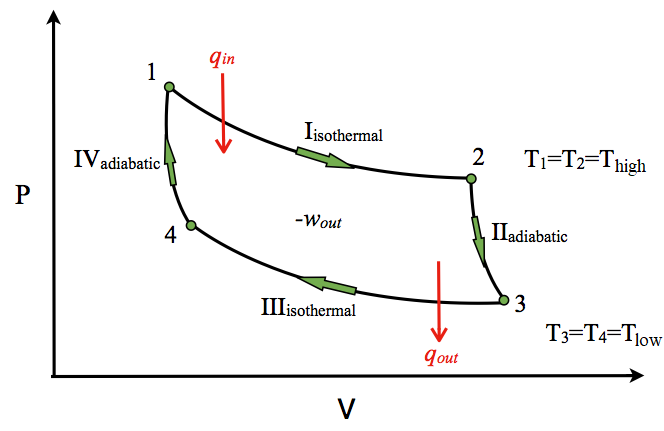
\includegraphics[width=0.7\linewidth]{Carnot better.png}
\end{figure}
The Carnot cycle describes a gas which, starting from point 1: is allowed to expand isothermally ($\Delta U=0$), doing work while absorbing heat $Q_{in}$ from a hot object or reservoir, to point 2; rapidly expands to point 3 with no heat exchange ($Q=0$), doing work; is made to contract isothermally to point 4 while losing heat ($Q_{out}$) to a cold reservoir; and finally is compressed rapidly and adiabatically ($Q=0$) back to point 1.  

In fact, there's nothing particularly special about the Carnot cycle, except that it's reversible and easy to analyze. It's reversible because we could just as easily do each step in reverse. In the isothermal steps, we just let the temperature stay constant as the piston moves the opposite way; and the adiabatic ($Q=0$) steps are very fast, with no friction or heat loss, so could (in theory) happen as many times as possible.

It's a bit complicated, but not that tricky, to show that the efficiency (work out divided by $Q_{in}$) of a Carnot cycle is $\frac{T_{high}-T_{low}}{T_{high}}$. What is very tricky and clever is Carnot's argument that (a) any other reversible process must have the same efficiency, and (b) no process of any kind could have a better efficiency. For, as we discussed in class, if there were a process which violated these conditions, we could combine it with a reversed Carnot cycle - a Carnot refrigerator, if you will - and perpetually move heat from a cold reservoir to a hot one. The machine would run forever, perpetually, and provide free refrigeration and work besides. I don't have time to repeat the full argument here, but it's all over the internet if you look.

The statement that no thermodynamic process could have a better efficiency than the Carnot limit is very strong. We seem to be talking about engines, but the theoretical framework here does not require pistons and chambers. We could imagine any process, and it won't be as efficient (in terms of extracting work) than Carnot. 

Remember though, the logic depends fundamentally on the premise that there is no perpetual motion, or equivalently, no way to make heat flow indefinitely from cold to hot. As long as we believe that, we have a theoretical limit on the percentage of thermal energy which can be converted into work, and therefore, any form of energy besides thermal. (It is worth noting that, unlike the Carnot cycle, many or most processes take in heat while the gas is changing $T$. So a little more work is required to deal with such a processes on a theoretical level; the approach is to consider the process in small steps, each of which could be connected to a reversed Carnot engine.) 

Put another, weaker way, Carnot's cycle shows that, for a fluid, you can never turn heat completely into work. This is true even though energy conservation suggests you could! This seems closely related to the idea we have been discussing about impossible processes like table molecules causing books to slide. The sliding book turned work (of whoever pushed it) completely into heat; the opposite process, of the table's heat turning into work to move the book, is impossible. 

Still though, couldn't a lot of the table's heat turn (inefficiently) into a little work, making the book slide just a little? Maybe? No. So despite having Carnot's theorem, we still have work to do in order to develop a theory of irreversibility, although we're making progress.

We didn't have a problem yet in this section, so in preparation for the next one:

\textbf{Problem 6*.} Show that $Q_{in}/T_{high}=Q_{out}/T_{low}$ for a Carnot cycle. Start from the following relations for the isothermal processes: $W_{12}=NkT_{high}\ln\frac{V_1}{V_2}$, and a similar one for $W_{34}$. Next, recall that $PV^\gamma$ is constant for adiabatic processes to show that $V_1/V_4=V_2/V_3$. Finally, use the First Law, equation 2, to derive the result.

7. \underline{Entropy and ``useful" energy}

Let's go back to the result of problem 6:  $Q_{in}/T_{high}=Q_{out}/T_{low}$ for a Carnot cycle. This means that the total change in $Q/T$ is zero for a Carnot process. This is because in step 12, it's $+Q_{in}/T_{high}$; in step 23, it's zero ($Q=0$); in step 34, it's $Q_{out}/T_{low}$, but this is a loss of heat and equals $-Q_{in}/T_{high}$ according to the previous problem; and finally for step 41, zero ($Q=0$ again).

For this reason, and I believe others, $Q/T$ was a quantity of interest in thermodynamic processes to a number of physicists, including Rudolf Clausius in the 1840s and 1850s. Because for most processes, $Q/T$ is not zero. Indeed, as a simple but critically important example:

\textbf{Problem 7.} Consider two large objects at different temperatures $T_{high}=400$ K and $T_{low}=300$ K. The objects are brought in contact and exchange $Q=100$ J of heat energy. This is not enough heat that the objects meaningfully change temperature, since they are so large, so we'll act like their $T$s stay constant (an approximation, but fine here).

\textbf{a.} Calculate the quantity $Q/T$ for each object, where $Q$ is negative for lost heat and positive for gained heat.

\textbf{b}. Show that the total amount of $Q/T$ ``of the universe" increased during this process.

\textbf{c}. Show that in general, when a small amount of heat flows from a hotter object to a colder one, the total change in $Q/T$ is positive although one object gains $Q/T$ and the other loses it.

Now, when the objects from problem 7 are at different temperatures, between them, there is a capacity do to work. Because, as we went over, the key prerequisite for a heat engine is a difference in pressure, and a difference in temperature is a sufficient condition to accomplish this. However, after they exchange heat for a long time, increasing $Q/T$, they eventually get to the same temperature. At least with respect to each other, they're no longer providing the capacity to do work.

For this reason, Clausius called this \textit{\textbf{entropy}}, from the Greek word for transformation, because Clausius figured out that a change in $S$ is related to a change in the capacity of an object or objects to do work. (He also stated that he wanted it to be similar to the word energy. So if this is confusing, blame Claudius.)

Like energy, entropy only really matters in terms of how much it changes. So a better definition of thermodynamic entropy is given in terms of its change: 
\begin{equation}
\Delta S = \frac{\Delta Q}{T}
\end{equation}
There is a little difficulty with this equation, and it is that temperatures generally change when heat flows. So in general as entropy is changing, $T$ is not constant, and the expression $\Delta Q/T$ does not allow us to calculate the change in $S$. Instead, we turn to calculus, and consider a very small amount of heat flow $dQ$. In this case, we have the best definition of thermodynamic entropy, in terms of its change: $dS = dQ/T$.

Later, it was discovered that the proper definition of entropy included a zero point $S=0$ at $T=0$. This is known as the Third Law of Thermodynamics, and it matters if you want to calculate absolute values of entropy, as chemists and others need to do. But we don't need to worry about the absolute amount of entropy for now, just the change.

Okay, so we now have a mathematical quantity, entropy, which increases when heat flows randomly from a hot object to a cold object; but stays constant in, for one example, the special case of a Carnot cycle, or more generally, any reversible thermodynamic cycle. And in fact, we can now see why the Carnot cycle is only theoretical. Because in reality, the expansion step 23 and the contraction step 41, which we called adiabatic, don't really have $Q=0$. There is always some heat flow; no system is completely isolated. And when heat flows, as we saw in the simple problem above, the total $S$ increases. 

What does that mean for our process? It means that, in the long run, we're losing the ability to produce work. Rather than the engine always accepting input energy at $T_{hot}$, and only emitting energy at $T_{cold}$, there is a leakage. Gradually, the cold area will become warmer, and the hot area will become cooler, and we'll lose our ability to generate work. Notice that the efficiency of a Carnot process when $T_{high}=T_{low}$ is zero!

So, if we design a thermodynamic process extremely carefully, we can get work out of thermal energy at something close to the Carnot efficiency, and have the universe's entropy increase only slowly; but if we don't take care, or just let a fluid evolve more or less randomly, then some work might happen, but at a lower efficiency than Carnot and where $S$ increases at a greater rate. There is no third option, where the total entropy decreases. If there were, the cycle's efficiency would be greater than the Carnot efficiency, and we could use it to power a perpetual motion engine or refrigerator.


In this sense, the amount of ``usable" energy in the universe - energy which can be converted into work, or non-thermal KE, or PE - is always decreasing. Because the only way to convert thermal energy to another form is if there is a difference in temperature; and spontaneous heat flow from hot to cold, or equivalently increases in entropy, always reduces this difference. No process in the universe seems to be exempt from this rule. It's the Second Law of Thermodynamics, and it's philosophically troubling. You can read in the Wolfram resource cited below that this consideration most definitely bothered Kelvin, Boltzmann, and surely many of the other leading figures in the history of thermodynamics.

Indeed, as $S$ continues to increase, and usable energy decrease, the universe would eventually (in a very long time) evolve into a state where everything is at the same (cold) temperature and nothing ever changes. $S$ would be at its maximum possible value. This scenario is known as the heat death of the universe. Based on thermodynamics, it seems possible. Then again, perhaps there are some higher powers or other processes which are beyond our current ability to scientifically understand.

Notice that, if you want to do work, heat is your friend. In today's news we're used to heat being the climate change enemy, but in terms of usable energy and the capacity to do work, it's just great that we are close to a giant ball of hot gas. 

In any case, regarding the heat death, it might make you feel better to review the result of the problem where you calculated the energies of the baseball. If you did it correctly, you found that there are orders of magnitude more thermal energy in the baseball than the kinetic energy is has when moving pretty fast. Now think about the thermal energy in the sun! Thermal energy is around, and there is a lot of it. It seems to be losing its ability to do work all the time, but that shouldn't really be a problem for billions and billions of years, to say the least. We happen to be living in a time of low entropy, or at least, low enough for lots of wonderful things to be possible. Wolfram has some more musings, in the references.

In any case, so it was that Clausius famously defined the First and Second Laws of Thermodynamics:

1. \textit{\textbf{First Law: the energy of the universe is constant}}

2. \textbf{\textit{Second Law: the entropy of the universe tends to a maximum.}}

Or as some say, tongue in cheek (but maybe not really):

1. First Law: you can't win

2. Second Law: you can't break even

The first law is a restatement of the conservation of energy, based on Newton's $F=ma$, with the understanding that heat is a flow of energy. The second law, however, to this point rests on a sort of axiom: heat won't flow from hot to cold on its own. Is there any weakness in this axiom? What is is based on?

8. \underline{From thermodynamic to statistical entropy}

As just mentioned, the Second Law has a weakness: it's based on an axiom about the direction of heat flow. So we need to dive into that a little bit. Why couldn't heat flow from a cold object to a hot object?

Well, the answer to that is what we discussed in class. Heat flow, at least via conduction, happens when molecules smash into each other and exchange energy. In molecular collisions, the total energy is conserved, but the less energetic molecule gains energy from the more energetic molecule (if the molecules are complicated, this may only be true in a statistical sense, but with large numbers of molecules it becomes a statistical certainty on average). Now, not every molecule in the ice has less energy than every molecule in the water; there is a range in each. And so it's possible that, if we consider only a few collisions, there were collisions of very energetic ice molecules with very slow water molecules, and some heat flowed from the ice to the water. But this can only happen up to a point. Eventually, it becomes a statistical certainty that the ice will get warmer and the water colder. (The other types of heat flow, convection and radiation, are also constrained by statistics in a similar way.)

So, it looks like the Second Law is a statistical statement; perhaps we need to look at irreversibility through a statistical lens. And Ludwig Boltzmann did exactly that. A brilliant theoretical physicist, Boltzmann developed an entire branch of physics, statistical mechanics, which explains a lot of what's happening with thermodynamics and irreversibility. Stat mech is the subject of an entire college semester course. That said I'll try to go through the basic basics here, for entropy.

Boltzmann's particular insight (in relation to entropy) was to think about a gas as a statistical distribution where the molecules have a certain probability of having positions $(x,y,z)$ in a small range near whatever arbitrary $\vec{x}$, and velocities $(v_x,v_y,v_z)$ in a small range around some arbitrary $\vec{v}$. You can see that the distribution depends the volume of the fluid, which determines how many particles are near whatever position; and on its energy, which determines how many particles have velocity in a certain range.  If the volume changes, like if we compress the gas, the distribution changes as more particles will be packed closer together. If the energy changes, like if we add heat, then the number of molecules whose velocity is near a given $\vec{v}$ will increase or decrease, depending on the temperature and the $\vec{v}$ in question.

As the particles move and collide according to $F=ma$, their individual positions and velocities change. However, at equilibrium (where all parts of the gas are at the same $T$), the statistical distribution of these quantities will not change. That is to say, there will always be roughly the same number of particles in each spatial area (assuming the fluid is contained), and there will always be roughly the same number of particles in a given velocity range.

What about systems in flux, which are not yet at equilibrium? In this case, the statistical distribution does change. Using some rather brilliant mathematics, beyond our scope, Boltzmann showed that during this change a certain function of the probability distribution of positions and speeds, known as the $H$-function, will always tend to a minimum (under the condition of a large number of random collisions conserving energy). The entropy was thought of as related to the inverse of the $H$-function, and therefore would go to a maximum. This was true for any change of state of the gas.

This ``proves" the Second Law, in the sense of showing that the classical $F=ma$ dynamics of collisions makes the system inevitably end up in a state of minimum $H$, which is to say, maximum entropy. And notices that a state of maximum entropy doesn't mean nothing is changing. The molecules are still bouncing around, changing position and exchanging kinetic energy. However, the statistical distribution of the positions and velocities is static, and so entropy is unchanging.

The distribution of positions at equilibrium is obviously uniform, if we ignore gravity. (If not, we get different densities at different depths, as in the real atmosphere - a fun problem! - and actually, it's by analogy with this situation that Feynman arrives at the Maxwell-Boltzmann in his lectures. But for now let's ignore gravity, which is okay if the fluid is small, without much vertical height to it.) 

What about the distribution of speeds? This is known as the Maxwell-Boltzmann distribution; it was derived independently by James Maxwell, without statistical mechanics, using the following ingenious argument:  Let $f(v_x)dv_x$ be the probability that a given molecule's $x$-direction velocity is between $v_x$ and $v_x+dv_x$. Since there was nothing special about the $x$ direction, motion along the $y$ and $z$ axes should follow the same distribution. Furthermore, motion along any axis is independent of the motion along the other two axes. So the probability that $\vec{v}$ lies in the range $(v_x+dv_x, v_y+dv_y, v_z+dv_z)$ equals $f(v_x)f(v_y)f(v_z)dv_xdv_ydv_z$. However, against because the axes are arbitrary, this probability can only depend on $|\vec{v}|$, or equivalently, $v^2$. The only function where $f(v_x)f(v_y)f(v_z)$ is a function of $v^2$ alone is $f(\vec{v})= Ce^{-\beta(v_x^2+v_y^2+v_z^2)}=Ce^{-\beta v^2}$. To find the value of $\beta$, do this problem:

\textbf{Problem 8*}. Consider a monatomic gas of $N$ molecules with fixed total thermal energy is $E$. The molecules' velocities are distributed according to a Maxwell distribution of the form $f(\vec{v})=Ce^{-\beta v^2}$.

\textbf{a.} The distribution must be normalized so that the total number of molecules, $\int f(\vec{v})d^3\vec{v}$, equals $N$. The integral runs from $-\infty$ to $\infty$ on each of $v_x$, $v_y$ and $v_z$. Show that as a result, $C=N\left( \frac{\beta}{\pi} \right)^{3/2}$. 

\textbf{b.} Show that the average velocity is zero.

\textbf{c.} Now we can calculate $\beta$ because we know the total KE, $\int \frac{1}{2}mv^2 f(\vec{v}) d^3\vec{v}$, equals $\frac{3}{2}NkT$. Do so to find $\beta$ and the Maxwell-Boltzmann distribution: 
\begin{equation}
f(\vec{v}) = N \left( \frac{m}{2\pi k T}\right)^{3/2} e^{-\frac{mv^2}{2kT}}
\end{equation}
This problem shows how the temperature $T$ is, in fact, the parameter of a statistical distribution; this is the best definition for temperature.

In summary, Boltzmann defined statistical entropy as a quantity which is maximized when a fluid achieves its equilibrium statistical distribution of positions and velocities. But we still don't have a mathematical expression, or really any kind of definition; the $H$-function is in general impossible to calculate analytically, and besides, only ordinally related to the entropy. 

9. \underline{The Boltzmann entropy}

To move to an actual expression for statistical entropy, let's look at another type of irreversible process we haven't considered before. A container for gas has two equal-sized compartments, separated by a valve. One is filled with $N$ molecules of helium gas, and the other is empty. At time $t=0$, the partition is removed:
\begin{figure}[h]
    \centering
    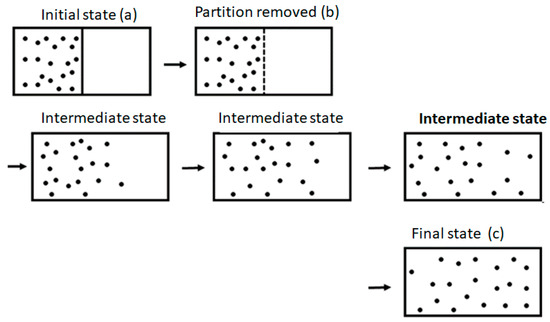
\includegraphics[width=0.5\linewidth]{entropy-box.jpg}

\end{figure}
Instead of 20 molecules in each side, imagine the box is a sort of tabletop size, so that there are actually a few moles, 20 trillion trillion or so, molecules! Then it's obvious, from a statistical standpoint, that pretty soon after $t=0$ and forever after that, there will be equal numbers of molecules, $N/2$, in each half.

\textbf{Problem 9.} When the valve has been open for a while, each molecule has a probability 1/2 to be on either side at a given moment (maybe we should say, if we wait for a long time, each molecule will spend 1/2 its time on the right and 1/2 on the left). 

\textbf{a.} Show that, after the valve has been open for a while and the gas is mixed, the probability that all $N$ of the He molecules end up on one side is $1/2^{N}$

\textbf{b.} Calculate this number for $N=10000$, and then for $N=10^{23}$. 

\textbf{c.} Calculate the probability that, after a long time, if $N=10^{23}$, 50.0001\% of the He particles are on the left side. (Use the binomial distribution, or a normal approximation - heh, should be pretty good here - or an online tool.)

This problem shows that the gas molecules will be evenly divided between both sides of the container forever; it is a statistical certainty. The container will never return to the way it was before we opened the valve, and this should be accounted for by entropy. 

Boltzmann realized that one way of looking at what changes when the valve is opened is that the molecules of each type suddenly have more ``accessible states" available to them. In this example, the new states are position states, specifically, all the locations in the right side of the container that the left side molecules can now access. It's clear that any time we give a gas more accessible positions, it will rush to fill them; and as long as there are a large number of molecules, it is a statistical certainty that the molecules will be more or less uniformly distributed throughout the available space, for all time.

A similar approach applies to the velocities of gas molecules. Adding heat to a gas means that the molecules are suddenly able to occupy more velocity states, because there is more energy to go around. So Boltzmann reasoned that entropy is related to the number of accessible states, meaning positions and velocities, that the gas can access, either because of the space it occupies (positions), or because of the energy it has (velocities). 

As far as the positions, clearly, the gas being uniformly distributed everywhere maximizes the number of possible positions which can be accessed by the gas molecules (if not, and they are clumped, then certain areas would be harder to access in the very short term). It's much less obvious with the velocities, because they are not uniformly distributed; but, and this is really the clincher, the Maxwell-Boltzmann distribution of velocities is the one which provides the maximum number of possible arrangements of velocities. That is to say, if we only have a certain amount of energy to divide up between the gas molecules, the MB distribution gives us the most options on how to do this. A "clumped" distribution of velocities would be one where a lot of molecules are slow, and a few very fast; this would leave too many middle states unreachable for most molecules, at least in the short term. If the velocities were uniformly distributed, then the energy constraint would leave some high speed states completely empty.

Let's use the example of the gas container with the valve to develop an expression for statistical entropy. We want the entropy to increase with the number of accessible states. The letter $\Omega$ is usually used to denote this number. So the statistical entropy should have the forme $S=f(\Omega)$ for some (monotonically) increasing function $f$. Which?

We can figure this out by examining the thermodynamics of the process and calculating $\Delta S=\Delta Q/T$ for the container.

\textbf{Problem 10.} Say the container with the removable partition from problem 9 is thermally sealed from the outside (it's made by Yeti, perhaps), so no heat flows in or out. The gas is initially on one side, and then the partition is removed.

\textbf{a.} Explain why the temperature of the gas must stay constant through the expansion.

\textbf{b.} Explain why $Q=-W$ for this expansion. 

\textbf{c*.} For an isothermal process, $P=NkT/V$. Use this and $W=\int P dV$ to show that $W=-NkT\ln 2$ for this expansion.

\textbf{d.} Now show that $\Delta S=Nk \ln 2$. Use the result of (c) even if you didn't derive it.

We are almost there. We know that the entropy change is $\Delta S = Nk \ln 2$. We also know that the number of accessible states went from $\Omega_1=CV^N$ to $\Omega_2=C(2V)^N$ for some $C$ when the volume available to the gas doubled. So the statistical version of entropy satisfies $\Delta S = f(2^N\Omega)-f(\Omega^N)= Nk \ln 2$. The monotonically increasing function which satisfies this relation is the logarithm. So it is that we arrive at the famous Boltzmann entropy:
\begin{equation}
S = k \ln \Omega.
\end{equation}

There is a lot to say about this equation; hopefully you will take statistical mechanics some day because this essay is long enough. For now, just one more thing: if I have two containers of gas, the first with $\Omega_1$ accessible states and the second with $\Omega_2$ accessible states, then the number of accessible states of the two containers together is $\Omega_1\Omega_2$, by combinatorics: for each state of container 1, the gas in container 2 can be in any of the $\Omega_2$ possible states. So the entropy of the two containers together is $S=k \ln \Omega_1\Omega_2 = k \ln \Omega_1+ k \ln \Omega_2 = S_1 + S_2$, where $S_1$ and $S_2$ are the entropies of each container by itself. This shows that entropy is an \textit{extensive} quantity, meaning, it scales with the size of the system. This should seem intuitively reasonable. 

One more fun problem: there is an old math puzzle which asks: which is bigger, $\pi^e$ or $e^\pi$? Of course this is easy with a calculator, but back in the day it wasn't so easy. There are some elegant proofs, and here is one based on entropy:

\textbf{Problem 11}. A small object A with temperature $\pi$ is brought in contact with a very large reservoir B, of temperature $e$. Heat flows until the temperatures are in equilibrium.

\textbf{a*}. If the small object A has heat capacity $C_V$ and mass $m$, so that $\delta U = mC_V\delta T$, show that A loses $mC_V(1- \ln \pi)$ of entropy. Use the thermodynamic expression.

\textbf{b}. The very large object B absorbs all the heat lost by the small object solid. Again using $\delta U = mC_V\delta T$ for the small solid, show that B gains $mC_V(\frac{\pi}{e}-1$ of entropy.

\textbf{c}. Since the total entropy change must be positive, by the Second Law, figure out which of $\pi^e$ and $e^\pi$ is larger.

10. \underline{Other ways of expressing entropy} - so many other ways

We're on page 14 here and we just talked about only 2 forms of entropy: statistical and thermodynamic. Ha - we're not even close to done. For one thing there is the famous Shannon entropy, which is critical to information theory and computer science. Among others:

\begin{figure}[h]
    \centering
    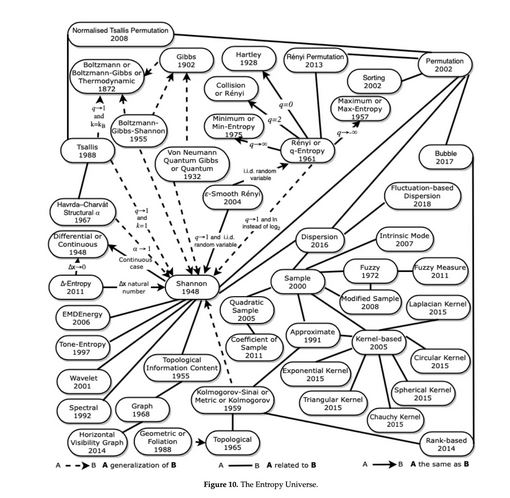
\includegraphics[width=0.7\linewidth]{entropy universe.JPG}
\end{figure}

Apparently, these are all the different ways in which people have conceived of entropy. It's a lot.

Here are some references. Happy reading!

https://www3.nd.edu/~powers/ame.20231/maxwell1872.pdf

https://www.wolframscience.com/reference/notes/1019b/

https://writings.stephenwolfram.com/2023/02/computational-foundations-for-the-second-law-of-thermodynamics/

https://writings.stephenwolfram.com/2023/01/how-did-we-get-here-the-tangled-history-of-the-second-law-of-thermodynamics/

https://girolami-group.chemistry.illinois.edu/publications/publications/J.\%20Chem.\%20Eng.\%20Data\%202020,\%2065,\%20298.pdf

https://www.perplex.ethz.ch/thermo\_course/various\_thermodynamics\_texts/Muller\%202007\%20A\%20history\%20of\%20thermodynamics.pdf

https://www.aps.org/apsnews/2015/06/joule-mechanical-equivalent-heat

https://www.1902encyclopedia.com/S/STE/steam-engine-01.html

(http://galileoandeinstein.physics.virginia.edu/more\_stuff/TeachingHeat.htm).

https://farside.ph.utexas.edu/teaching/plasma/Plasma/node35.html

\end{document}